%pgfplot test
% \documentclass{article}
% \usepackage{pgfplots}
% \begin{document}
% Preamble: 
% \pgfplotsset{width=7cm,compat=1.14}
% \begin{tikzpicture}
% \begin{axis}[
% hide x axis,
% hide y axis
% ]
% \addplot [red]{sin(deg(x))};
% \addplot [green]{cos(deg(x))};
% \end{axis}

% \begin{axis}[enlarge x limits=false]
% \addplot [red,samples=500] {sin(deg(x))};
% \addplot [orange,samples=7] {sin(deg(x))};
% \addplot [teal,const plot,samples=14]
% {sin(deg(x))};
% \end{axis}
% \end{tikzpicture}% <- eliminate space.
% \end{document}

% None: f(x) = sin(20x)
% AM: f(x) = cos(.5x)∙sin(20∙x)
% FM: f(x) = cos(20∙x+15∙sin(x)+10)

\documentclass[border=10pt]{standalone} 
\usepackage{pgfplots}
\pgfplotsset{%
	compat=1.14,
% 	axis line style={draw=none},
% 	tick style={draw=none},
% 	xticklabels=\empty,
% 	yticklabels=\empty,
% % 	domain=0:500,
% 	samples=300,
% 	hide axis, 
% 	scale only axis,
% 	width=1in,
% 	height=0.2in,
}
\begin{document}
{
% \begin{tikzpicture} % No modulation
%    \begin{axis}[grid=none,scale=1, restrict y to domain=-1:1]
%      \addplot[blue, smooth, unbounded coords=discard,line join=round, line cap=round]plot (\x, { sin(1500*\x) });
%    \end{axis}
% \end{tikzpicture}
% 
% \begin{tikzpicture} %AM
%    \begin{axis}[grid=none,scale=1]
%      \addplot[black, smooth, unbounded coords=discard,line join=round, line cap=round]plot (\x, { cos(60 * \x) * sin(1500 * \x) });
%    \end{axis}
% \end{tikzpicture}

   \newcommand{\nCF}{80}%Carrier Frequency
   \newcommand{\nLF}{40}%Lowest Frequency

\pgfplotsset{%
% 	axis line style={draw=none},
% 	tick style={draw=none},
% 	xticklabels=\empty,
% 	yticklabels=\empty,
% % 	domain=0:500,
	samples=1e3,
	clip=false,
% 	hide axis, 
% 	scale only axis,
	width=5in,
	height=2in,
	domain=0:3*pi,%degrees per cycle * number of cycles (show 50 cycles of the carrier)
	%
	axis line style={draw=none},
	tick style={draw=none},
	xticklabels=\empty,
	yticklabels=\empty,
% 	hide axis, 
}


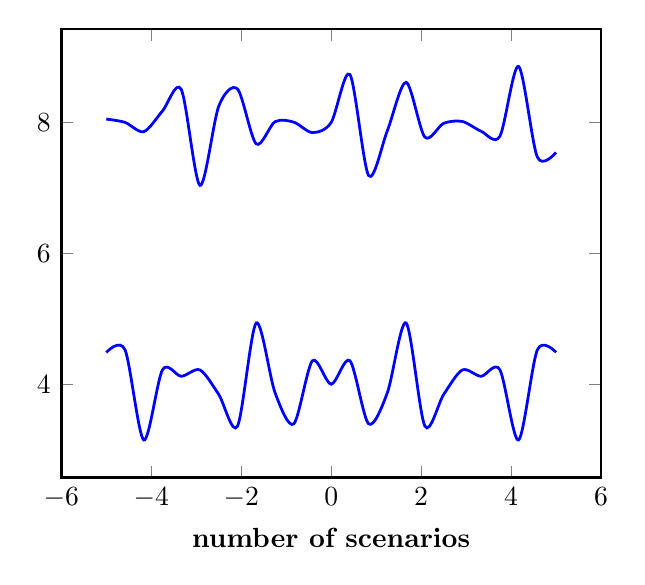
\begin{tikzpicture}
\begin{axis}[xlabel = \textbf{number of scenarios},	line width=1pt,
]

% 	\addplot [red,  smooth,domain=0:36,] {cos((30.0*deg(\x))+(15.0*sin(deg(\x)))+0.5)};
% 	\addplot [blue, smooth,domain=0:36,] {2+cos(30.0*deg(\x)/(1+\x/(66)))};%sweep
% 	\addplot [green,smooth,domain=0:36,] {4+sin(20*deg(x))};
% 	\addplot[domain=0:15,red,samples=2000] {cos((x*20 + 6*sin(x*2*180/pi))*180/pi)};%FM
% 	https://tex.stackexchange.com/questions/440425/animated-cosine-waveform-with-fm-modulation-using-the-animate-package-part-2
% 	\addplot[green, smooth, domain=0:15,samples=2000] {((cos(x*2*180/pi)+1))};%FM control
% 
% 	\addplot[red, smooth] {sin(x*20*180/pi)+6};%no modulation - working
	\addplot[blue, smooth] {sin(x*20*180/pi)*sin(x*1*180/pi)+4};%AM-working
% 	\addplot[purple, smooth] {sin((x*20 + 6*(sin(x*2*180/pi)))*180/pi)+2};%FM-working
	\addplot[blue, smooth] {0.5*sin(x*20*180/pi)*(1+sin(x*1.7*180/pi))+8};%AM-test
\end{axis}
\end{tikzpicture}


% \begin{tikzpicture} % FM
%    \begin{axis}[hide axis=false]
% % 	\addplot[green, smooth, samples=1e3, domain=-20:20, unbounded coords=discard,line join=round, line cap=round]plot (\x, { cos(20 * \x + 15 * sin(\x)) });
% 	\addplot[red,smooth]plot (\x,   { sin(\x)});%carrier
% 	\addplot[blue,smooth]plot (\x,   { sin(\x)});%carrier
% % 	\addplot[blue,smooth]plot (\x,  { sin(\x/10)});%every 15 cycles of the carrier
% % 	\addplot[green,smooth]plot (\x, { (sin(\x/10)*4.5)+8});%carrier modulated by a sin wave
% % 	\addplot[blue,smooth]plot (\x,  { sin(\x/((sin(\x/15)*7)+8))});%every 15 cycles of the carrier
%    \end{axis}
% \end{tikzpicture}

%Rainbow colored sine wave
%formula M*sin(A*x+B*(x^2)/C)
%A=Start frequency
%B=End frequency-Start frequency
%C=number of samples
%M=multiplying height factor since we need smaller pgfplots height than allowed.
% \newcommand{\nA}{10}% Start frequency.
% \newcommand{\nB}{110}% End frequency - start frequency.
% \newcommand{\nC}{.1e3}% Number of samples.
% \newcommand{\nM}{0.5}% Multiplying factor for amplitude.
% 
% \pgfplotsset{
% 	colormap={bluered}{
% 		rgb255(0cm)=(128,0,0); rgb255(1cm)=(255,0,0); rgb255(2cm)=(255,255,0);
% 		rgb255(3cm)=(100,255,0);rgb255(4cm)=(0,255,255); rgb255(5cm)=(0,0,180)},
% 	domain=1:\nC
% }
% 
% \begin{tikzpicture}[rotate=90]
% 	\begin{axis}[width=11in,height=1in]
% 		% http://www.fon.hum.uva.nl/praat/manual/Script_for_creating_a_frequency_sweep.html
% 		\addplot [black,line width=3pt,line join=round, line cap=round]             {\nM * sin(\nA * x + \nB * (x^2) / \nC)};
% 		\addplot [mesh,point meta=x,line width=2pt,line join=round, line cap=round] {\nM * sin(\nA * x + \nB * (x^2) / \nC)};
% 	\end{axis}
% \end{tikzpicture}
}
\end{document}
